% Workshop paper (candidate venues: LLM4Code, AIware, an ICSE/FSE workshop on AI-assisted SE). Venue not final.
\PassOptionsToPackage{expansion=false}{microtype}% bitmap fallback fonts cannot be expanded when libertine is missing
\documentclass[sigconf]{acmart}
\usepackage{booktabs}
\usepackage{tikz}
\usetikzlibrary{positioning,arrows.meta,fit,backgrounds}
\newcommand{\nPRs}{11,996}
\newcommand{\nMerged}{8,211}
\newcommand{\baseLine}{10.8}
\newcommand{\baseFile}{3.2}
\newcommand{\nLines}{9.2M}
\newcommand{\nFiles}{463,599}
\newcommand{\nPass}{2}
\newcommand{\nChecks}{8}
\newcommand{\undoneBareSuppression}{12.1}
\newcommand{\faBareSuppression}{2.1}
\newcommand{\flagsBareSuppression}{26.6}
\newcommand{\undoneCommentedOutCode}{12.3}
\newcommand{\faCommentedOutCode}{5.4}
\newcommand{\flagsCommentedOutCode}{105.3}
\newcommand{\undoneScopeCi}{2.1}
\newcommand{\faScopeCi}{2.7}
\newcommand{\flagsScopeCi}{29.8}
\newcommand{\undoneScopeGitignore}{3.2}
\newcommand{\faScopeGitignore}{3.9}
\newcommand{\flagsScopeGitignore}{10.0}
\newcommand{\undoneScopeLockfile}{4.1}
\newcommand{\faScopeLockfile}{2.5}
\newcommand{\flagsScopeLockfile}{5.1}
\newcommand{\undoneScopeNewDoc}{12.4}
\newcommand{\faScopeNewDoc}{1.7}
\newcommand{\flagsScopeNewDoc}{9.0}
\newcommand{\undoneScopeUnrelated}{4.0}
\newcommand{\faScopeUnrelated}{16.3}
\newcommand{\flagsScopeUnrelated}{812.7}
\newcommand{\undoneWorkaroundComment}{15.8}
\newcommand{\faWorkaroundComment}{4.3}
\newcommand{\flagsWorkaroundComment}{20.6}
\newcommand{\aSampled}{300}
\newcommand{\aReachable}{295}
\newcommand{\aWithInstructionFiles}{135}
\newcommand{\aWithRules}{134}
\newcommand{\aRules}{14,710}
\newcommand{\aReposWithUnenforcedCheckableRule}{61}
\newcommand{\aEnforced}{20}
\newcommand{\aEnforcedPct}{0.1}
\newcommand{\aEnforceable}{209}
\newcommand{\aEnforceablePct}{1.4}
\newcommand{\aJudgment}{14,481}
\newcommand{\aJudgmentPct}{98.4}
\newcommand{\lPRs}{862}
\newcommand{\lMerged}{612}
\newcommand{\lMaxChars}{14,000}
\newcommand{\lBase}{11.3}
\newcommand{\lSec}{1.6}
\newcommand{\lTokIn}{2.98M}
\newcommand{\lTokOut}{0.26M}
\newcommand{\lTokPerPR}{3.7k}
\newcommand{\lTrTwoPct}{2}
\newcommand{\lTrTwoFlags}{2.2}
\newcommand{\lTrTwoUndone}{15.8}
\newcommand{\lTrTwoFa}{0.8}
\newcommand{\lTrTwoN}{19}
\newcommand{\lTrAllPct}{18}
\newcommand{\lTrAllFlags}{36.8}
\newcommand{\lTrAllUndone}{5.1}
\newcommand{\lTrAllFa}{11.1}
\newcommand{\lTrAllN}{317}
\newcommand{\lLlmSamePct}{55}
\newcommand{\lLlmSameFlags}{88.2}
\newcommand{\lLlmSameUndone}{12.1}
\newcommand{\lLlmSameFa}{32.1}
\newcommand{\lLlmSameN}{760}
\newcommand{\lLlmAllPct}{88}
\newcommand{\lLlmAllFlags}{257.1}
\newcommand{\lLlmAllUndone}{9.2}
\newcommand{\lLlmAllFa}{48.6}
\newcommand{\lLlmAllN}{2,216}

\setcopyright{none}
\acmConference[Workshop submission]{Under review}{2026}{venue to be decided}
\settopmatter{printacmref=false}
\renewcommand\footnotetextcopyrightpermission[1]{}
\renewcommand{\showeprint}[2][]{}
\begin{document}\sloppy
\title{Stop Reviewing the Same Mistake Twice:\\ Measuring Deterministic Checks and an LLM Reviewer on Coding-Agent Pull Requests}
\author{Harshul Jain}\affiliation{\institution{Independent Researcher}\city{}\country{}}
\begin{abstract}
Teams write rules for coding agents in prose files such as \texttt{AGENTS.md}, and reviewers keep correcting the same mistakes in agent pull requests (PRs). We present Trellis, an open-source command-line tool and GitHub Action that audits which written rules nothing enforces, scans agent PRs for common scope and slop problems, and ratchets new debt, with no LLM. We evaluate its eight built-in checks on \nPRs{} multi-commit agent PRs from AIDev, counting a flag as \emph{undone} when the same PR later removes what it flagged. Against a pass bar fixed before the run (at least 5\% undone, at most 3 false-alarm PRs per 100), only \nPass{} of \nChecks{} checks pass: new summary documents (\undoneScopeNewDoc\% undone, \faScopeNewDoc{} false alarms per 100 PRs) and unexplained suppressions (\undoneBareSuppression\%, \faBareSuppression). On \lPRs{} PRs that both could read in full, an LLM reviewer (Claude Haiku) flags \lLlmAllPct\% of PRs, its flags are undone \lLlmAllUndone\% of the time (line baseline \lBase\%), and on \lLlmAllFa{} of every 100 PRs none of its flags led to a change; Trellis's two passing checks flag \lTrTwoPct\% of PRs at \lTrTwoFa{} false alarms per 100. An audit of \aSampled{} repositories finds that \aReposWithUnenforcedCheckableRule{} of \aWithRules{} with extractable agent rules have at least one checkable rule that nothing enforces. Neither reviewer predicts corrections much better than chance on this proxy; the difference is noise.
\end{abstract}
\keywords{coding agents, code review, static analysis, AGENTS.md, LLM reviewers, review debt}
\maketitle

\section{Introduction}
Coding agents now open hundreds of thousands of PRs on GitHub~\cite{li2026aidev}, and reviewing them has become the bottleneck. Teams steer agents with context files such as \texttt{AGENTS.md}, \texttt{CLAUDE.md} and \texttt{.cursor/rules}~\cite{chatlatanagulchai2025agentreadmes}. These files are prose: an agent can ignore them, and a human has to notice when it does. Lauren Tan's talk \emph{All Code Is Slop (Except Mine)}~\cite{tan2026slop} argues that a repeated correction should become structure, a lint rule, a type, a test, rather than another line of instructions, and Cursor's \texttt{/correct} skill~\cite{pstack} does this interactively. Trellis is the CI half of that idea.

Two cheaper alternatives exist. Teams can add more prose, or they can put an LLM reviewer on every PR~\cite{greptilebench}. Benchmarks of LLM reviewers measure how many known bugs they find~\cite{sweprbench,ccrab,greptilebench} but rarely how often their comments are noise, which is what a team pays for on every PR. We ask three questions:
\begin{description}
\item[RQ1] Do the problems a deterministic scanner flags in agent PRs get corrected more often than ordinary lines?
\item[RQ2] Is an LLM reviewer, given the same problem classes, better at flagging what gets corrected, and at what noise and cost?
\item[RQ3] How many written agent rules could be checks but are not?
\end{description}
Our contributions are the tool (\S\ref{sec:tool}), an order-independent \emph{undone} measure for AIDev, which has no commit order (\S\ref{sec:method}), and results that are mostly negative for both reviewers (\S\ref{sec:results}). Code, scripts and raw results are public.

\section{Related Work}
\textbf{Static analysis and ratchets.} Linters and rule engines~\cite{semgrep} are effective when developers trust them, and false positives are the main reason they are ignored~\cite{johnson2013why,sadowski2018lessons}. Betterer~\cite{betterer} and reviewdog~\cite{reviewdog} restrict checks to new code. Trellis reuses both ideas and targets problems typical of agent PRs.
\textbf{Agent PRs.} AIDev~\cite{li2026aidev} collects agent-authored PRs; studies of why they fail~\cite{ehsani2026fail} and of agent context files~\cite{chatlatanagulchai2025agentreadmes} motivate our checks. AI-to-AI review is already common~\cite{ai2ai}.
\textbf{LLM reviewers.} SWE-PRBench reports that frontier models find 15--31\% of human-flagged issues~\cite{sweprbench}; c-CRAB~\cite{ccrab} and a vendor benchmark~\cite{greptilebench} score bug catch rates without scoring noise. We score both reviewers with the same noise-aware measure.

\section{Trellis}\label{sec:tool}
\begin{figure}[t]\centering\footnotesize
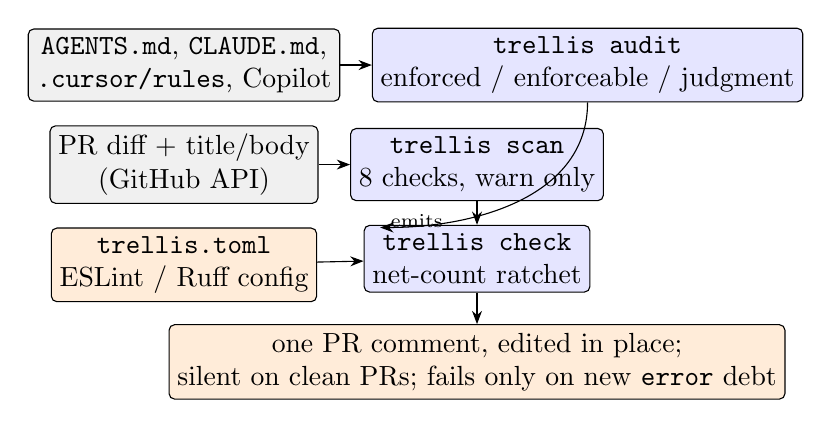
\begin{tikzpicture}[node distance=3mm and 4mm, box/.style={draw, rounded corners=2pt, align=center, inner sep=3pt, fill=#1}, box/.default=white, >=Stealth]
\node[box=gray!12] (rules) {\texttt{AGENTS.md}, \texttt{CLAUDE.md},\\ \texttt{.cursor/rules}, Copilot};
\node[box=blue!10, right=of rules] (audit) {\texttt{trellis audit}\\ enforced / enforceable / judgment};
\node[box=gray!12, below=of rules] (pr) {PR diff + title/body\\ (GitHub API)};
\node[box=blue!10, right=of pr] (scan) {\texttt{trellis scan}\\ 8 checks, warn only};
\node[box=blue!10, below=of scan] (check) {\texttt{trellis check}\\ net-count ratchet};
\node[box=orange!15, below=of pr] (cfg) {\texttt{trellis.toml}\\ ESLint / Ruff config};
\node[box=orange!15, below=4mm of check] (comment) {one PR comment, edited in place;\\ silent on clean PRs; fails only on new \texttt{error} debt};
\draw[->] (rules) -- (audit); \draw[->] (pr) -- (scan); \draw[->] (cfg) -- (check);
\draw[->] (audit.south) to[out=-90,in=0] node[pos=0.75,left,font=\scriptsize]{emits} ([xshift=8mm]cfg.north east);
\draw[->] (scan) -- (check); \draw[->] (check) -- (comment);
\end{tikzpicture}
\caption{Trellis. \texttt{audit} turns prose rules into configuration; \texttt{scan} and \texttt{check} run on each PR and the Action posts one comment. No LLM and no PR code is executed.}\label{fig:arch}
\end{figure}
Figure~\ref{fig:arch} shows the three commands. \textbf{\texttt{audit}} finds instruction files (16 path patterns), splits them into directive sentences and classifies each rule as \emph{enforced} (an existing ESLint, Ruff, import-linter or Trellis config checks it), \emph{enforceable} (Trellis recognizes the rule and emits the config that would check it) or a \emph{judgment} call. \textbf{\texttt{scan}} needs no configuration. It inspects added lines and changed files, skips generated, vendored and lock files, and has eight checks: workaround comments, suppressions with no reason, commented-out code, and five scope checks (lockfile without manifest, unexplained \texttt{.gitignore} and CI changes, new summary documents, and files outside the paths the PR names). \textbf{\texttt{check}} counts each rule's occurrences added minus removed, so moved code is not new debt, and fails only when an \texttt{error} rule gets worse. The \textbf{Action} reads configuration from the base branch and the diff from the API, never runs PR code, and edits only comments written by a bot or its own token.

\section{Method}\label{sec:method}
\textbf{Data.} We sampled \nPRs{} agent PRs with at least two commits from AIDev (seed 0; \nMerged{} merged). PRs with one commit (40\% of AIDev) cannot show a correction and are excluded.
\textbf{Undone.} AIDev records a PR's commits but not their order, so we sum over them. For each file and distinct line text we count how often the PR adds and removes it. A line flag is \emph{undone} when the text is removed at least as often as it is added; a file flag is undone when the PR's changes to the file cancel out. Lines are also rewritten in ordinary iteration, so each rate is compared with the same measure over all \nLines{} distinct added code lines (\baseLine\%) and \nFiles{} changed files (\baseFile\%).
\textbf{False alarms.} A false alarm is a merged PR in which none of a reviewer's flags were undone, counted once per PR and reported per 100 sampled PRs. This is an upper bound, because some surviving flags were real problems the team accepted.
\textbf{Pass bar.} Fixed before the run: a check stays on by default only with at least 5\% undone and at most 3 false-alarm PRs per 100.
\textbf{LLM reviewer.} We gave Claude Haiku (\texttt{claude-haiku-5-5}, thinking off) each PR's title, description and commit patches, described the eight Trellis classes plus a ninth for any other defect, and asked for JSON naming the file and the exact added line. We kept PRs whose patches fit in \lMaxChars{} characters so both reviewers see the same full input (\lPRs{} PRs with a valid reply, \lMerged{} merged). Flags quoting a line the PR never added were dropped. Spending was capped before the run.
\textbf{Audit.} We ran \texttt{audit} on \aSampled{} random non-fork AIDev repositories through the GitHub API.

\section{Results}\label{sec:results}
\begin{table}[t]\centering\caption{RQ1: \texttt{trellis scan} on \nPRs{} agent PRs. Undone with 95\% Wilson CI; FA/100 = false-alarm PRs per 100 PRs. Baselines: \baseLine\% of lines, \baseFile\% of files.}\label{tab:scan}
\footnotesize\setlength{\tabcolsep}{3pt}\resizebox{\columnwidth}{!}{\begin{tabular}{lrrrl}\toprule
Check & Flags/100 & Undone \% [95\% CI] & FA/100 & \\\midrule
New summary/notes document & 9.0 & 12.4 [10.5, 14.5] & 1.7 & pass \\
Suppression with no reason & 26.6 & 12.1 [11.0, 13.3] & 2.1 & pass \\
Lockfile without manifest & 5.1 & 4.1 [2.8, 6.0] & 2.5 & fail \\
CI config change & 29.8 & 2.1 [1.7, 2.6] & 2.7 & fail \\
\texttt{.gitignore} change & 10.0 & 3.2 [2.3, 4.3] & 3.9 & fail \\
Workaround comment & 20.6 & 15.8 [14.4, 17.3] & 4.3 & fail \\
Commented-out code & 105.3 & 12.3 [11.8, 12.9] & 5.4 & fail \\
File outside named paths & 812.7 & 4.0 [3.9, 4.2] & 16.3 & fail \\
\bottomrule\end{tabular}
}\end{table}
\begin{figure}[t]\centering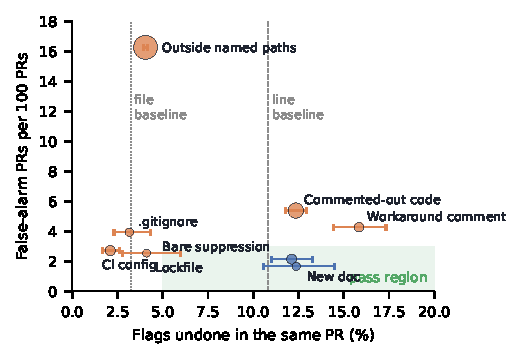
\includegraphics[width=\columnwidth]{../figures/fig_checks.pdf}
\caption{Each check against the pass bar. Bubble size: flags per 100 PRs; whiskers: 95\% CI. Blue checks pass.}\label{fig:checks}\end{figure}
\textbf{RQ1: two of eight checks pass.} Table~\ref{tab:scan} and Figure~\ref{fig:checks} show the results. New summary documents are undone \undoneScopeNewDoc\% of the time, nearly four times the file baseline, at \faScopeNewDoc{} false alarms per 100 PRs. Unexplained suppressions (\undoneBareSuppression\%, \faBareSuppression) also pass. Workaround comments (\undoneWorkaroundComment\%) and commented-out code (\undoneCommentedOutCode\%) are undone more often than ordinary lines but leave too many merged PRs with surviving flags. Lockfile, \texttt{.gitignore} and CI checks sit at or below the baseline, and the out-of-scope check fires \flagsScopeUnrelated{} times per 100 PRs. Following the bar, we recommend that only the two passing checks comment by default.

\begin{figure*}[t]\centering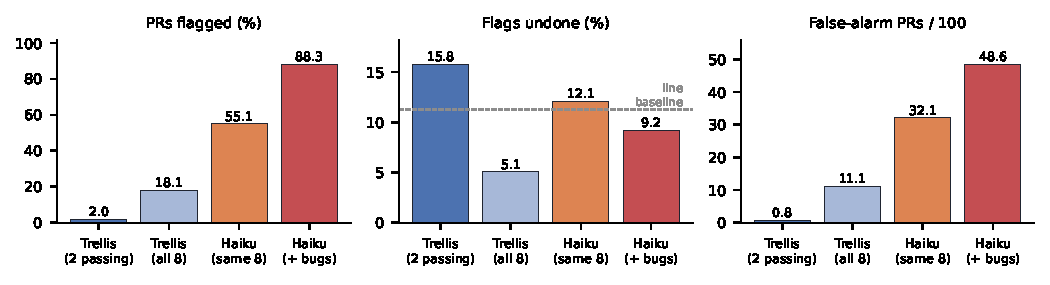
\includegraphics[width=\textwidth]{../figures/fig_llm.pdf}
\caption{RQ2: Trellis and Claude Haiku on the same \lPRs{} PRs, scored identically. Dashed line: share of all added code lines undone on this subset (\lBase\%).}\label{fig:llm}\end{figure*}
\begin{table}[t]\centering\caption{RQ2 numbers behind Figure~\ref{fig:llm}.}\label{tab:llm}
\footnotesize\setlength{\tabcolsep}{3pt}\resizebox{\columnwidth}{!}{\begin{tabular}{lrrrr}\toprule
Reviewer & PRs flagged \% & Flags/100 & Undone \% & FA/100 \\\midrule
Trellis, the two passing checks & 2 & 2.2 & 15.8 & 0.8 \\
Trellis, all eight checks & 18 & 36.8 & 5.1 & 11.1 \\
Haiku, the same eight classes & 55 & 88.2 & 12.1 & 32.1 \\
Haiku, all issues incl.\ bugs & 88 & 257.1 & 9.2 & 48.6 \\
\bottomrule\end{tabular}
}\end{table}
\textbf{RQ2: the LLM is not better, and is much noisier.} Haiku flags \lLlmAllPct\% of PRs (Figure~\ref{fig:llm}, Table~\ref{tab:llm}). Its flags are undone \lLlmAllUndone\% of the time, below the \lBase\% rate for any added line, and on \lLlmAllFa{} of every 100 PRs none of them led to a change. Restricted to Trellis's eight classes it is undone more often than Trellis's full set (\lLlmSameUndone\% vs.\ \lTrAllUndone\%) but leaves \lLlmSameFa{} false-alarm PRs per 100 against \lTrAllFa. Trellis's two passing checks flag \lTrTwoPct\% of PRs at \lTrTwoFa{} false alarms per 100, but rest on only \lTrTwoN{} flags. Haiku used about \lTokPerPR{} tokens and \lSec\,s per PR; Trellis runs offline in milliseconds. On this proxy neither reviewer predicts corrections much better than chance. The practical difference is noise: a quiet deterministic check costs a reviewer almost nothing to read.

\begin{figure*}[t]\centering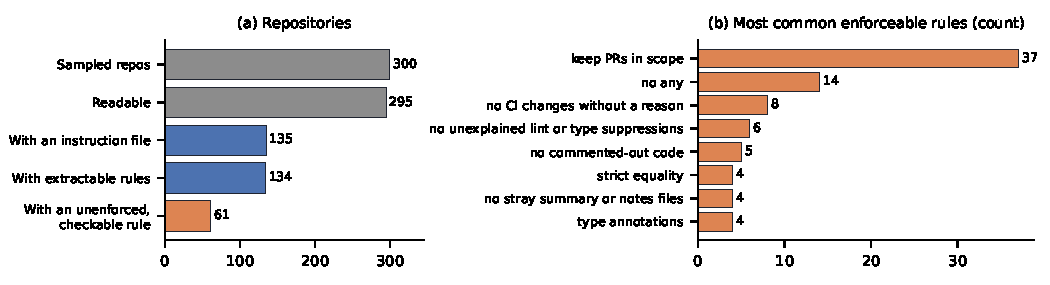
\includegraphics[width=\textwidth]{../figures/fig_audit.pdf}
\caption{RQ3: \texttt{trellis audit} on \aSampled{} AIDev repositories. (a) How many repositories have agent rules and unenforced checkable rules. (b) The most common enforceable rules.}\label{fig:audit}\end{figure*}
\textbf{RQ3: written rules that could be checks.} Of \aReachable{} readable repositories, \aWithInstructionFiles{} have an instruction file and \aWithRules{} have extractable rules (\aRules{} in total; Figure~\ref{fig:audit}). \aReposWithUnenforcedCheckableRule{} of them have at least one rule that nothing enforces and that Trellis could turn into a check; the most common are keeping PRs in scope, banning \texttt{any} and explaining CI changes. Only \aEnforcedPct\% of extracted rules are enforced and \aEnforceablePct\% enforceable; \aJudgmentPct\% are judgment calls, partly because the extractor treats every bullet as a rule.

\section{Limitations}
\emph{Undone} is a proxy for corrected: it ignores order, cannot see corrections made in a later PR, and counts accepted problems as false alarms, so false-alarm rates are upper bounds. Logic bugs an LLM raises may be fixed by edits to other lines, which this proxy misses. The LLM comparison uses one model, one prompt and smaller PRs. The two passing checks rest on few flags in the LLM subset. Audit uses patterns, not an LLM, and treats lint configuration as repository-wide. We have not yet validated the proxy against human judgment.

\section{Ethics}
All data are public GitHub activity released in AIDev; we report aggregates only. Trellis runs locally or in CI, needs no API key and never executes PR code.

\section{Conclusion}
A deterministic scanner can catch a few kinds of agent-PR slop quietly, and most of its candidate checks fail a noise bar fixed in advance. An LLM reviewer given the same classes is not better at predicting corrections and comments on most PRs. Both results argue for measuring reviewer noise, not only catch rate, before putting any reviewer on every PR. Trellis, the scripts and the raw results are at \url{https://github.com/harshuljain13/rd0-trellis}; it is the second tool in rd0, a family of tools that reduce review debt from agent PRs.

\bibliographystyle{ACM-Reference-Format}
\bibliography{../refs}
\end{document}
